%\documentclass{cmspaper}
%\begin{document}

\section{Event Selection} \label{sec:eventSelection}

% Analysis strategy (M dist, bump search)
% Optimize signal, minimize bkgd
% Plots of selection variables
% (optimization of selection criteria)
% List of selection criteria (Mee, St, etc.)

The basic strategy to identify the existence of a particle that decays to a jet and an electron 
is to study the invariant mass of the electron-jet pairs in the events. 
The signal of a leptoquark would appear as a bump in the distribution of this invariant mass.
The decay of a particle to a jet and a lepton is forbidden in the standard model.  
Thus, a peak at the mass of the leptoquark would be the only resonance in this distribution. 
The electron-jet combinations of the background events have a different shape than that 
of the leptoquark resonance. 
Nonetheless, the number of background events could dominate over the number of signal events.  
The cut-based selection described in this section has been made in order to minimize the number 
of background events selected while retaining a high signal efficiency.

The decay of a leptoquark and an anti-leptoquark produces two high energy electrons and 
two high energy jets.
The online selection of candidate events is made by either the HLT trigger ``HLT\_Photon15\_L1R'' 
or ``HLT\_Photon25\_L1R'' described in section~\ref{sec:trig}, depending on the luminosity scenario, 
while the offline identification of electrons and jets 
proceeds as described in sections~\ref{sec:electrons} and \ref{sec:jet}, respectively.

%FIXME add skim
In order to reduce the size of the of the data samples and the time to analyze them, a skim of the 
data has been defined.
The requirements that the skim has to satisfy have been defined considering that this skim may be needed
for the analysis of both first and second generation leptoquark pair production. Such requirements are:
\begin{itemize}
\item having a high efficiency for first (events with 2 electrons and 2 jets) and second (events with 
2 muons and 2 jets) generation leptoquark pair production;
\item keeping events needed for the control samples: the control sample for the Z+jets background is $Z\rightarrow l l$+ 2 jets,
where $l$ is is either an electron or a muon; the control sample for the the $t\bar{t}$+jets background is a sample 
with an electron, a muon and 2 jets;
\item suppress all other backgrounds
\end{itemize}
The definition of the skim has been chosen as:
\begin{itemize}
\item $N_l \equiv N_e + N_{\mu} \ge 2$, where $N_e (N_{\mu})$ is the number of reconstructed electrons (muons)
with $P_T>20~$GeV and no extra ID or isolation requirements applied.
\item 
\item 
\item 
\end{itemize}




The offline selection of the eejj sample continues with the following kinematical cuts:
%
\begin{enumerate}
\item at least 2 isolated electrons, both of them required $P_T>30$~GeV 
\item at least 2 jets, both of them required to have $P_T>50$~GeV
\item $M_{ee}>100$~GeV
\item $S_T\equiv P_T(e_1)+P_T(e_2)+P_T(j_1)+P_T(j_2)>f(M_{LQ})$, where $f(M_{LQ})$ is a function 
of the hypothesized LQ mass.
\end{enumerate}
%

The specific values of the kinematical cuts has been determined using a cut-optimization procedure meant to
reach the maximum potential of the analysis for excluding the existence of a LQ signal. 
Such a procedure is described in section~\ref{sec:optimization}.

Cut 2 and 3 set a minimum value on the transverse momentum of electrons and jets.
Cut 3, where $M_{ee}$ is the invariant mass of the electron pair, removes background events from 
$Z/\gamma$+jets events as shown in figure~\ref{fig:Mee_St_distributions}-left.
Cut 4, where the variable $S_T$ is defined as the scalar sum of the transverse momenta of the 
2 electrons and 2 jets, is applied following the approach of the experiment $D0$ in 
\cite{Abazov:2001mx}. In that paper, an event selection optimization as a function of
the combinations of several kinematic variables has shown that $S_T$ is the most powerful one 
and little is gained by adding cuts on other variables. The distribution of $S_T$ for the present
analysis is shown in figure~\ref{fig:Mee_St_distributions}-right.

Once the eejj sample is selected, there are two ways to combine two electrons and two jets to make two electron-jet pairs. 
For each event, the combination with the minimum difference, $\Delta M_{ej}$, between the invariant masses, $M_{ej}$, 
of the two electron-jet pairs is chosen. 
The resulting $M_{ej}$ distribution is shown in figure~\ref{fig:Mej_allComb} for the signal and remaining backgrounds. 
FIXME   A detailed study of the optimization of the selection criteria, and of alternative algorithms to identify the best candidate 
electron-jet combinations, will be performed in future upgrades of this analysis.

\begin{figure}[htbp]
  \begin{center}
    \begin{tabular}{cc}
      \resizebox{7.5cm}{!}{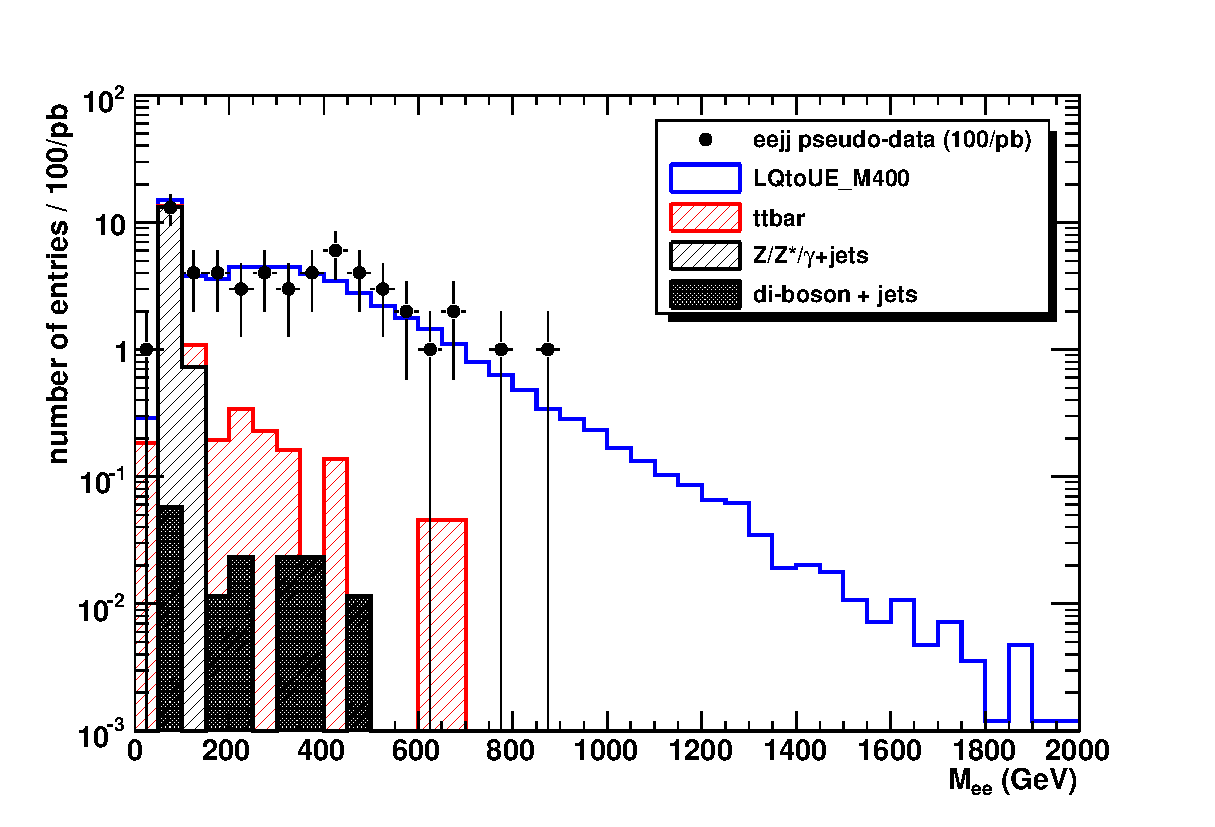
\includegraphics{plots/LQ400FullSimeejjFinalPlots/Mee_eejj_LQ400_100pb.eps}} &
      \resizebox{7.5cm}{!}{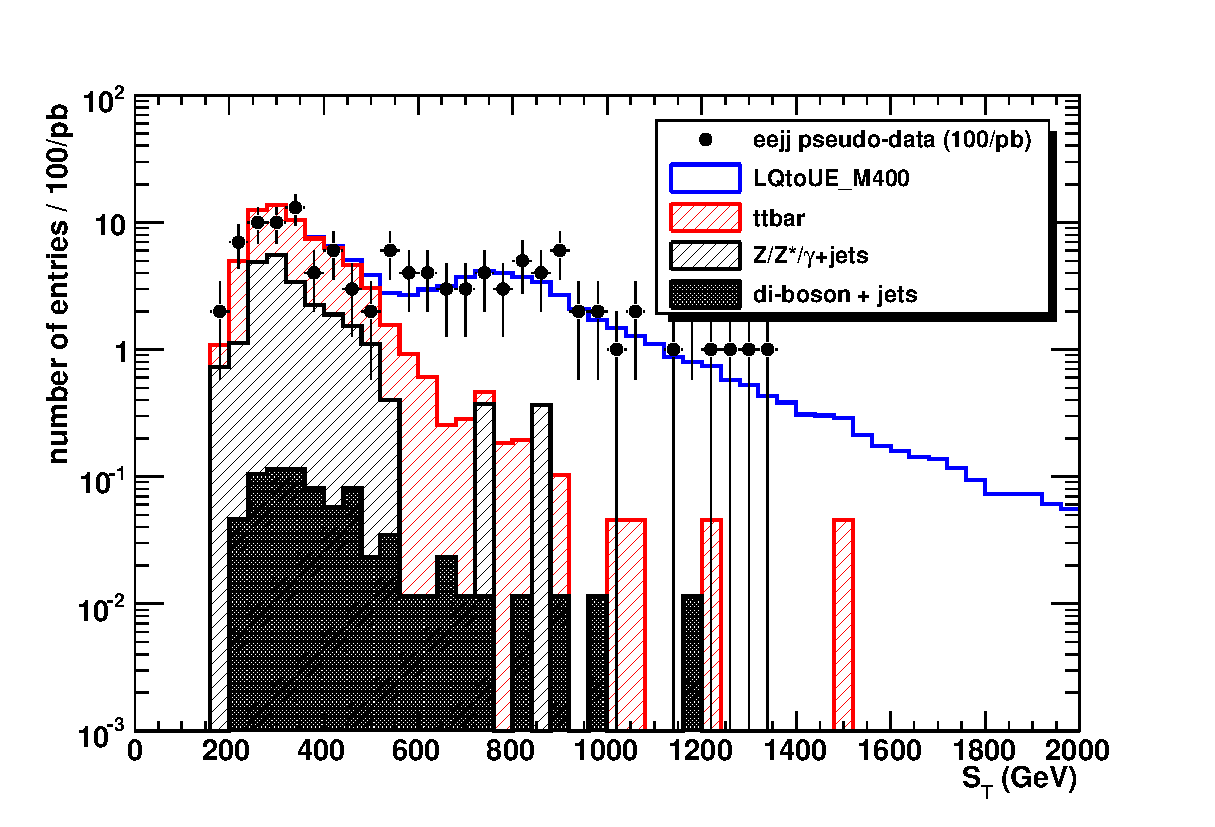
\includegraphics{plots/LQ400FullSimeejjFinalPlots/ST_eejj_LQ400_100pb.eps}} \\
    \end{tabular}
    \caption{\small \sl Left: invariant mass of the electron pair, $M_{ee}$. 
             Right: scalar sum of the $P_T$ of the 2 leading electrons and 2 leading jets. 
	     In each histogram, the distributions for the signal (for leptoquark mass 250 and 650~GeV) and the 
	     relevant backgrounds are shown after applying all cuts except the one involving the 
	     plotted variable. 
	     All histograms are summed on top of each other.
	     FIXME - comment on QCD not included.}
    \label{fig:Mee_St_distributions}
  \end{center}
\end{figure}


\begin{figure}[htbp]
  \begin{center}
    \begin{tabular}{cc}
      \resizebox{7.5cm}{!}{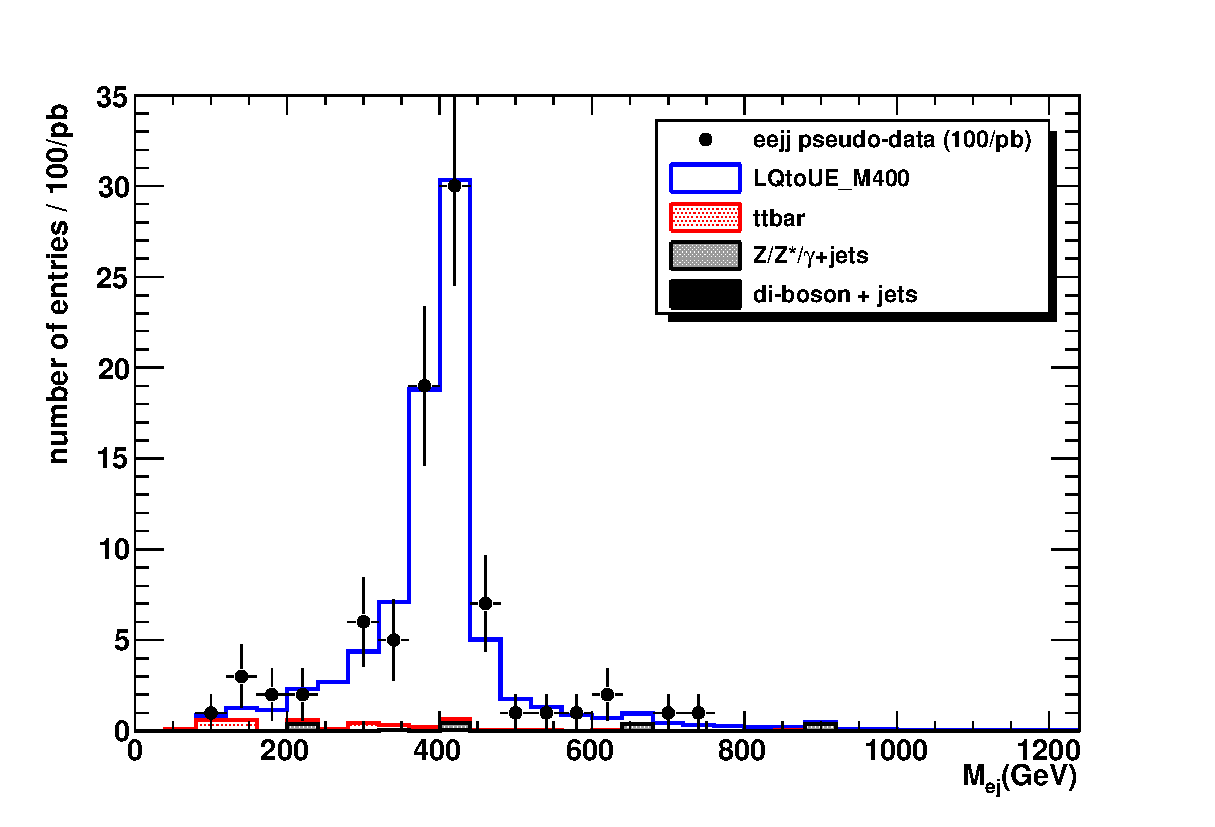
\includegraphics{plots/LQ400FullSimeejjFinalPlots/Mej_eejj_LQ400_100pb_LinScale.eps}} & 
      \resizebox{7.5cm}{!}{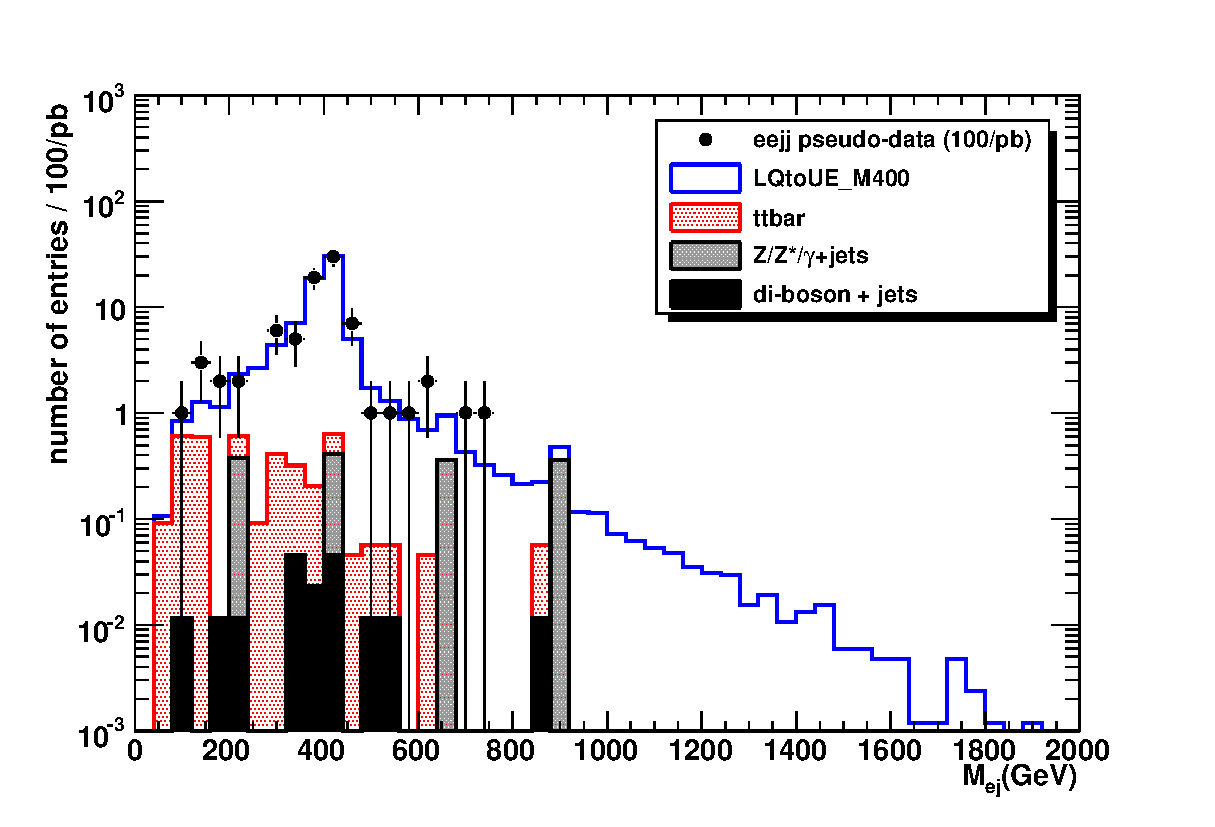
\includegraphics{plots/LQ400FullSimeejjFinalPlots/Mej_eejj_LQ400_100pb.eps}} \\
    \end{tabular}
    \caption{\small \sl Distribution of the invariant mass, $M_{ej}$, 
      of the electron-jet pairs 
      with smaller $\Delta M_{ej}$
      for signal at 400~GeV and backgrounds (in linear and log scale on the left- and right-hand-side, respectively). 
      The complete event selection has been applied.
      All histograms are summed on top of each other.
      FIXME- comment on QCD not included}
    \label{fig:Mej_allComb}
  \end{center}
\end{figure}


Tables  
\ref{tab:effic-MLQ400}, 
\ref{tab:effic-ttbar}, 
\ref{tab:effic-Z}, 
\ref{tab:effic-QCD},
\ref{tab:effic-VV} and
\ref{tab:effic-W}
show the efficiency of the selection cuts for signal events at $M_{LQ}=400~$GeV and the main background samples.
In all these tables, the $S_T$ cut is set to the value (620~GeV) optimized for this LQ mass.  

\begin{table}[htbp] 
\begin{center} 
\begin{tabular}{|c|c|c|c|} 
\hline\hline 
 Cut & $N_{evt}$ passed for $100pb^{-1}$ & $\varepsilon_{rel}$ & $\varepsilon_{abs}$ \\ 
\hline\hline 
None          &           7.500e+01          $~\pm~$          0.000e+00           &           1.000e+00          $~\pm~$          0.000e+00           &           1.000e+00          $~\pm~$          0.000e+00          \\          
          Skim          &           6.804e+01          $~\pm~$          9.000e-02           &           9.072e-01          $~\pm~$          1.323e-03           &           9.100e-01          $~\pm~$          1.200e-03          \\          
          2 ele $P_T>20~$GeV          &           6.769e+01          $~\pm~$          9.000e-02           &           9.949e-01          $~\pm~$          1.875e-03           &           9.000e-01          $~\pm~$          1.200e-03          \\          
          2 ele (ID) $P_T>20~$GeV          &           5.826e+01          $~\pm~$          1.200e-01           &           8.607e-01          $~\pm~$          2.452e-03           &           7.800e-01          $~\pm~$          1.700e-03          \\          
          2 ele (ID+Iso) $P_T>20~$GeV          &           5.065e+01          $~\pm~$          1.400e-01           &           8.694e-01          $~\pm~$          3.447e-03           &           6.800e-01          $~\pm~$          1.900e-03          \\          
          2 ele (ID+Iso) $P_T>30~$GeV          &           5.009e+01          $~\pm~$          1.400e-01           &           9.889e-01          $~\pm~$          3.931e-03           &           6.700e-01          $~\pm~$          1.900e-03          \\          
          2 jets (Cleaned) $P_T>20~$GeV          &           4.968e+01          $~\pm~$          1.400e-01           &           9.918e-01          $~\pm~$          3.969e-03           &           6.600e-01          $~\pm~$          1.900e-03          \\          
          2 jets (Cleaned), $P_T>50~$GeV, $ | \eta |<3$          &           4.662e+01          $~\pm~$          1.400e-01           &           9.384e-01          $~\pm~$          4.118e-03           &           6.200e-01          $~\pm~$          1.900e-03          \\          
          $M_{ee}>100~$GeV          &           4.460e+01          $~\pm~$          1.500e-01           &           9.567e-01          $~\pm~$          4.509e-03           &           5.900e-01          $~\pm~$          2.000e-03          \\          
          $ S_T>620~$GeV           &           3.880e+01          $~\pm~$          1.500e-01           &           8.700e-01          $~\pm~$          5.124e-03           &           5.200e-01          $~\pm~$          2.000e-03          \\          
          \hline\hline 
\end{tabular} 
\end{center} 
\caption{Sample of $M_{LQ}=400~$GeV (FullSim): Sequence of selection cuts with number of events selected in 100$~pb^{-1}$, efficiency relative to the preceeding cut and absolute efficiency.} 
\label{tab:effic-MLQ400} 
\end{table} 

\begin{table}[htbp] 
\begin{center} 
\begin{tabular}{|c|c|c|c|} 
\hline\hline 
 Cut & $N_{evt}$ passed for $100pb^{-1}$ & $\varepsilon_{rel}$ & $\varepsilon_{abs}$ \\ 
\hline\hline 
None          &           4.140e+04          $~\pm~$          0.000e+00           &           1.000e+00          $~\pm~$          0.000e+00           &           1.000e+00          $~\pm~$          0.000e+00          \\          
          Skim          &           6.745e+03          $~\pm~$          1.607e+01           &           1.629e-01          $~\pm~$          2.382e-03           &           1.600e-01          $~\pm~$          3.900e-04          \\          
          2 ele $P_T>20~$GeV          &           3.637e+03          $~\pm~$          1.232e+01           &           5.392e-01          $~\pm~$          4.141e-03           &           8.800e-02          $~\pm~$          3.000e-04          \\          
          2 ele (ID) $P_T>20~$GeV          &           4.621e+02          $~\pm~$          4.570e+00           &           1.271e-01          $~\pm~$          1.045e-02           &           1.100e-02          $~\pm~$          1.100e-04          \\          
          2 ele (ID+Iso) $P_T>20~$GeV          &           2.578e+02          $~\pm~$          3.420e+00           &           5.579e-01          $~\pm~$          1.655e-02           &           6.200e-03          $~\pm~$          8.300e-05          \\          
          2 ele (ID+Iso) $P_T>30~$GeV          &           1.549e+02          $~\pm~$          2.660e+00           &           6.010e-01          $~\pm~$          2.169e-02           &           3.700e-03          $~\pm~$          6.400e-05          \\          
          2 jets (Cleaned) $P_T>20~$GeV          &           1.473e+02          $~\pm~$          2.590e+00           &           9.510e-01          $~\pm~$          2.457e-02           &           3.600e-03          $~\pm~$          6.300e-05          \\          
          2 jets (Cleaned), $P_T>50~$GeV, $ | \eta |<3$          &           7.619e+01          $~\pm~$          1.870e+00           &           5.171e-01          $~\pm~$          3.019e-02           &           1.800e-03          $~\pm~$          4.500e-05          \\          
          $M_{ee}>100~$GeV          &           4.562e+01          $~\pm~$          1.440e+00           &           5.988e-01          $~\pm~$          3.998e-02           &           1.100e-03          $~\pm~$          3.500e-05          \\          
          $ S_T>620~$GeV           &           1.460e+00          $~\pm~$          2.600e-01           &           3.200e-02          $~\pm~$          1.809e-01           &           3.500e-05          $~\pm~$          6.300e-06          \\          
          \hline\hline 
\end{tabular} 
\end{center} 
\caption{Sample of $t\bar{t}$ + N jets: Sequence of selection cuts with number of events selected in 100$~pb^{-1}$, efficiency relative to the preceeding cut and absolute efficiency.} 
\label{tab:effic-ttbar} 
\end{table} 

\begin{table}[htbp] 
\begin{center} 
\begin{tabular}{|c|c|c|c|} 
\hline\hline 
 Cut & $N_{evt}$ passed for $100pb^{-1}$ & $\varepsilon_{rel}$ & $\varepsilon_{abs}$ \\ 
\hline\hline 
None          &           4.218e+05          $~\pm~$          0.000e+00           &           1.000e+00          $~\pm~$          0.000e+00           &           1.000e+00          $~\pm~$          0.000e+00          \\          
          Skim          &           9.015e+03          $~\pm~$          5.667e+01           &           2.137e-02          $~\pm~$          6.286e-03           &           2.100e-02          $~\pm~$          1.300e-04          \\          
          2 ele $P_T>20~$GeV          &           4.168e+03          $~\pm~$          3.876e+01           &           4.624e-01          $~\pm~$          1.122e-02           &           9.900e-03          $~\pm~$          9.200e-05          \\          
          2 ele (ID) $P_T>20~$GeV          &           3.300e+03          $~\pm~$          3.453e+01           &           7.918e-01          $~\pm~$          1.400e-02           &           7.800e-03          $~\pm~$          8.200e-05          \\          
          2 ele (ID+Iso) $P_T>20~$GeV          &           3.092e+03          $~\pm~$          3.343e+01           &           9.369e-01          $~\pm~$          1.504e-02           &           7.300e-03          $~\pm~$          7.900e-05          \\          
          2 ele (ID+Iso) $P_T>30~$GeV          &           2.015e+03          $~\pm~$          2.702e+01           &           6.518e-01          $~\pm~$          1.722e-02           &           4.800e-03          $~\pm~$          6.400e-05          \\          
          2 jets (Cleaned) $P_T>20~$GeV          &           1.582e+03          $~\pm~$          2.395e+01           &           7.849e-01          $~\pm~$          2.022e-02           &           3.800e-03          $~\pm~$          5.700e-05          \\          
          2 jets (Cleaned), $P_T>50~$GeV, $ | \eta |<3$          &           3.244e+02          $~\pm~$          1.086e+01           &           2.051e-01          $~\pm~$          3.675e-02           &           7.700e-04          $~\pm~$          2.600e-05          \\          
          $M_{ee}>100~$GeV          &           2.293e+01          $~\pm~$          2.890e+00           &           7.069e-02          $~\pm~$          1.304e-01           &           5.400e-05          $~\pm~$          6.800e-06          \\          
          $ S_T>620~$GeV           &           7.300e-01          $~\pm~$          5.200e-01           &           3.184e-02          $~\pm~$          7.234e-01           &           1.700e-06          $~\pm~$          1.200e-06          \\          
          \hline\hline 
\end{tabular} 
\end{center} 
\caption{Sample of $Z/\gamma$ + N jets: Sequence of selection cuts with number of events selected in 100$~pb^{-1}$, efficiency relative to the preceeding cut and absolute efficiency.} 
\label{tab:effic-Z} 
\end{table} 

\begin{table}[htbp] 
\begin{center} 
\begin{tabular}{|c|c|c|c|} 
\hline\hline 
 Cut & $N_{evt}$ passed for $100pb^{-1}$ & $\varepsilon_{rel}$ & $\varepsilon_{abs}$ \\ 
\hline\hline 
None          &           1.541e+09          $~\pm~$          0.000e+00           &           1.000e+00          $~\pm~$          0.000e+00           &           1.000e+00          $~\pm~$          0.000e+00          \\          
          Skim          &           1.294e+06          $~\pm~$          7.932e+03           &           8.397e-04          $~\pm~$          6.128e-03           &           8.400e-04          $~\pm~$          5.100e-06          \\          
          2 ele $P_T>20~$GeV          &           9.947e+05          $~\pm~$          6.686e+03           &           7.684e-01          $~\pm~$          9.096e-03           &           6.500e-04          $~\pm~$          4.300e-06          \\          
          2 ele (ID) $P_T>20~$GeV          &           5.933e+03          $~\pm~$          5.834e+02           &           5.965e-03          $~\pm~$          9.855e-02           &           3.800e-06          $~\pm~$          3.800e-07          \\          
          2 ele (ID+Iso) $P_T>20~$GeV          &           1.768e+02          $~\pm~$          1.125e+02           &           2.981e-02          $~\pm~$          6.436e-01           &           1.100e-07          $~\pm~$          7.300e-08          \\          
          2 ele (ID+Iso) $P_T>30~$GeV          &           1.209e+02          $~\pm~$          1.099e+02           &           6.835e-01          $~\pm~$          1.109e+00           &           7.800e-08          $~\pm~$          7.100e-08          \\          
          2 jets (Cleaned) $P_T>20~$GeV          &           1.209e+02          $~\pm~$          1.099e+02           &           1.000e+00          $~\pm~$          1.285e+00           &           7.800e-08          $~\pm~$          7.100e-08          \\          
          2 jets (Cleaned), $P_T>50~$GeV, $ | \eta |<3$          &           1.155e+01          $~\pm~$          1.083e+01           &           9.556e-02          $~\pm~$          1.306e+00           &           7.500e-09          $~\pm~$          7.000e-09          \\          
          $M_{ee}>100~$GeV          &           7.400e-01          $~\pm~$          5.200e-01           &           6.407e-02          $~\pm~$          1.172e+00           &           4.800e-10          $~\pm~$          3.400e-10          \\          
          $ S_T>620~$GeV           &           3.700e-01          $~\pm~$          3.700e-01           &           5.000e-01          $~\pm~$          1.222e+00           &           2.400e-10          $~\pm~$          2.400e-10          \\          
          \hline\hline 
\end{tabular} 
\end{center} 
\caption{Sample of QCD ($H_T \in [100,1000]~$GeV): Sequence of selection cuts with number of events selected in 100$~pb^{-1}$, efficiency relative to the preceeding cut and absolute efficiency.} 
\label{tab:effic-QCD} 
\end{table} 

\begin{table}[htbp] 
\begin{center} 
\begin{tabular}{|c|c|c|c|} 
\hline\hline 
 Cut & $N_{evt}$ passed for $100pb^{-1}$ & $\varepsilon_{rel}$ & $\varepsilon_{abs}$ \\ 
\hline\hline 
None          &           1.180e+03          $~\pm~$          0.000e+00           &           1.000e+00          $~\pm~$          0.000e+00           &           1.000e+00          $~\pm~$          0.000e+00          \\          
          Skim          &           6.312e+01          $~\pm~$          8.300e-01           &           5.349e-02          $~\pm~$          1.315e-02           &           5.300e-02          $~\pm~$          7.100e-04          \\          
          2 ele $P_T>20~$GeV          &           2.321e+01          $~\pm~$          5.100e-01           &           3.677e-01          $~\pm~$          2.561e-02           &           2.000e-02          $~\pm~$          4.400e-04          \\          
          2 ele (ID) $P_T>20~$GeV          &           1.500e+01          $~\pm~$          4.100e-01           &           6.463e-01          $~\pm~$          3.507e-02           &           1.300e-02          $~\pm~$          3.500e-04          \\          
          2 ele (ID+Iso) $P_T>20~$GeV          &           1.377e+01          $~\pm~$          4.000e-01           &           9.180e-01          $~\pm~$          3.989e-02           &           1.200e-02          $~\pm~$          3.400e-04          \\          
          2 ele (ID+Iso) $P_T>30~$GeV          &           9.490e+00          $~\pm~$          3.300e-01           &           6.892e-01          $~\pm~$          4.531e-02           &           8.000e-03          $~\pm~$          2.800e-04          \\          
          2 jets (Cleaned) $P_T>20~$GeV          &           6.970e+00          $~\pm~$          2.800e-01           &           7.345e-01          $~\pm~$          5.313e-02           &           5.900e-03          $~\pm~$          2.400e-04          \\          
          2 jets (Cleaned), $P_T>50~$GeV, $ | \eta |<3$          &           1.580e+00          $~\pm~$          1.400e-01           &           2.267e-01          $~\pm~$          9.729e-02           &           1.300e-03          $~\pm~$          1.100e-04          \\          
          $M_{ee}>100~$GeV          &           7.800e-01          $~\pm~$          1.000e-01           &           4.937e-01          $~\pm~$          1.558e-01           &           6.600e-04          $~\pm~$          8.100e-05          \\          
          $ S_T>620~$GeV           &           9.000e-02          $~\pm~$          3.000e-02           &           1.154e-01          $~\pm~$          3.571e-01           &           7.900e-05          $~\pm~$          2.800e-05          \\          
          \hline\hline 
\end{tabular} 
\end{center} 
\caption{Sample of $VV$ + N jets: Sequence of selection cuts with number of events selected in 100$~pb^{-1}$, efficiency relative to the preceeding cut and absolute efficiency.} 
\label{tab:effic-VV} 
\end{table} 

\begin{table}[htbp]
\begin{center}
\begin{tabular}{|c|c|c|c|}
\hline\hline
 Cut & $N_{evt}$ passed for $100pb^{-1}$ & $\varepsilon_{rel}$ & $\varepsilon_{abs}$ \\
\hline\hline
None          &           4.560e+06          $~\pm~$          0.000e+00           &           1.000e+00          $~\pm~$          0.000e+00           &           1.000e+00          $~\pm~$
    0.000e+00          \\
          Skim          &           4.699e+03          $~\pm~$          5.920e+01           &           1.031e-03          $~\pm~$          1.260e-02           &           1.000e-03          $~\
pm~$          1.300e-05          \\
          2 ele $P_T>20~$GeV          &           2.344e+03          $~\pm~$          4.183e+01           &           4.989e-01          $~\pm~$          2.184e-02           &           5.100e-0
4          $~\pm~$          9.200e-06          \\
          2 ele (ID) $P_T>20~$GeV          &           1.284e+02          $~\pm~$          9.790e+00           &           5.478e-02          $~\pm~$          7.829e-02           &           2.8
00e-05          $~\pm~$          2.100e-06          \\
          2 ele (ID+Iso) $P_T>20~$GeV          &           2.240e+01          $~\pm~$          4.090e+00           &           1.744e-01          $~\pm~$          1.979e-01           &
 4.900e-06          $~\pm~$          9.000e-07          \\
          2 ele (ID+Iso) $P_T>30~$GeV          &           8.210e+00          $~\pm~$          2.480e+00           &           3.665e-01          $~\pm~$          3.530e-01           &
 1.800e-06          $~\pm~$          5.400e-07          \\
          2 jets (Cleaned) $P_T>20~$GeV          &           6.720e+00          $~\pm~$          2.240e+00           &           8.185e-01          $~\pm~$          4.498e-01           &
   1.500e-06          $~\pm~$          4.900e-07          \\
          2 jets (Cleaned), $P_T>50~$GeV, $ | \eta |<3$          &           1.490e+00          $~\pm~$          1.060e+00           &           2.217e-01          $~\pm~$          7.856e-01
       &           3.300e-07          $~\pm~$          2.300e-07          \\
          $M_{ee}>100~$GeV          &           0.000e+00          $~\pm~$          0.000e+00           &           0.000e+00          $~\pm~$          7.114e-01           &           0.000e+00
         $~\pm~$          0.000e+00          \\
          $ S_T>620~$GeV           &           0.000e+00          $~\pm~$          0.000e+00           &           0.000e+00          $~\pm~$          0.000e+00           &           0.000e+00
        $~\pm~$          0.000e+00          \\
          \hline\hline
\end{tabular}
\end{center}
\caption{Sample of W + N jets: Sequence of selection cuts with number of events selected in 100$~pb^{-1}$, efficiency relative to the preceeding cut and absolute efficiency.}
\label{tab:effic-W}
\end{table}



A summary of the number of selected signal and background events expected in 100 pb$^{-1}$ of data 
is reported in Table \ref{tab:EventSelSummary}. 
The overall signal selection efficiencies are around 30-50\% for the LQ masses investigated. 
After the described event selection, the dominant background contributions 
are $t\bar{t}$ and $Z/\gamma$+jets. Data-driven techniques to estimate these backgrounds
are discussed in section~\ref{sec:bkgStudy}.

\begin{table}[htbp]
\begin{center}
\begin{tabular}{|ccc||cccc|}
\hline\hline
Signal Samples       & $S_T$ cut       & Number of Events     & Number              & of Events           & in Background    & Samples     \\
                     & (GeV)           & in Signal Samples     & $t\bar{t}$ + N jets & $Z/\gamma$ + N jets & QCD              & VV + N jets \\ 
\hline
$M_{LQ}=250~$GeV     & 460             & 342.06 $\pm$ 2.10    & 7.18  $\pm$ 0.57    & 2.55  $\pm$ 0.96    & 0.37 $\pm$ 0.37  & 0.21 $\pm$ 0.05 \\ 
$M_{LQ}=250~$GeV (*) & 460             & 359.39 $\pm$ 1.36    & as above            & as above            & as above         & as above        \\
$M_{LQ}=300~$GeV (*) & 520             & 163.37 $\pm$ 0.53    & 3.89  $\pm$ 0.42    & 1.09  $\pm$ 0.63    & 0.37 $\pm$ 0.37  & 0.15 $\pm$ 0.04 \\ 
$M_{LQ}=400~$GeV     & 620             &  38.80 $\pm$ 0.15    & 1.46  $\pm$ 0.26    & 0.73  $\pm$ 0.52    & 0.37 $\pm$ 0.37  & 0.09 $\pm$ 0.03 \\ 
$M_{LQ}=400~$GeV (*) & 620             &  40.41 $\pm$ 0.10    & as above            & as above            & as above         & as above        \\
$M_{LQ}=500~$GeV (*) & 740             &  11.56 $\pm$ 0.03    & 0.69  $\pm$ 0.18    & 0.36  $\pm$ 0.36    & 0.00 $\pm$ 0.00  & 0.05 $\pm$ 0.02 \\ 
$M_{LQ}=600~$GeV (*) & 740             &   4.04 $\pm$ 0.01    & as above            & as above            & as above         & as above        \\
$M_{LQ}=650~$GeV (*) & 740             &   2.43 $\pm$ 0.01    & as above            & as above            & as above         & as above        \\
$M_{LQ}=700~$GeV (*) & 740             &   1.49 $\pm$ 0.00    & as above            & as above            & as above         & as above        \\
%$M_{LQ}=800~$GeV (*) & 740             &   0.59 $\pm$ 0.00    & as above            & as above            & as above         & as above        \\
%$M_{LQ}=900~$GeV (*) & 740             &   0.25 $\pm$ 0.00    & as above            & as above            & as above         & as above        \\
%$M_{LQ}=1000~$GeV (*)& 740             &   0.11 $\pm$ 0.00    & as above            & as above            & as above         & as above        \\
\hline\hline
\end{tabular}
\end{center}
\caption{\small \sl Number events expected from LQ signal and background samples after the analysis selection for 100 pb$^{-1}$ of data.
The value cut on the kinematic variable $S_T$ depends on the LQ mass, and it is indicated in the second column.
Data samples from FullSim Monte Carlo are used for all backgrounds and for LQ massed of 250 and 400 GeV. Signal samples marked by (*) are
made with the FastSim Monte Carlo.
The LQ cross section rapidly falls at high LQ mass, thus producing a relative decrease in the number of selected events. } 
\label{tab:EventSelSummary}
\end{table}

%FIXME explain here or elsewhere why we stop increasing sT cut?

%\end{document}
